\subsection{Implementering af accelerometre}
%Et accelerometer er en elektromekanisk enhed, som både kan måle statisk og dynamisk accerleration. Den statiske acceleration kan være tyngdekraften, hvor det er muligt at bestemme orienteringen af accelerometeret i forhold til jorden. De dynamiske kræfter såsom bevægelse, stød og vibrationer, gør det muligt at analysere accelerometeres bevægelse samt hastighed. 

I dette projekt anvendes der på baggrund af krav opstillet i \autoref{sec:acc_teori} to accelerometre ADXL335Z fra Analog Devices. Accelerometerne er en 3-aksialt sensor, som har et arbejdsområde på minimum $\pm~3~g$, og en spænding som output. Det analoge outputsignal er proportionalt med accelerationen \citep{analogdevices2009}. 

\noindent
Accelerometrene har en single-supply spændingsforsyning, som skal ligge mellem $1,8~-~3,6~V$.  Offsettet er afhængig af spændingen i spændingsforsyningen, da spændingen er $3,4~V$, bliver offsettet $1,7~V$, som er det halve af spændingsforsyningen. Båndbredden og støjen varierer for akserne. For x- og y-aksen ligger båndbredden mellem $0,5 - 1.600~Hz$ og støjen normalt på $150~\mu g/\sqrt{Hz}$ RMS. \fxnote{Den spektrale effekttæthed måles i $\mu g/$. Hvis dette divideres med kvadratroden af båndbredden af signalet $\sqrt{Hz}$, fås RMS af accelerationsstøjen ved en temperatur på $25^\circ$C} \citep{analogdevices2010}. %mens båndbredden for z-aksen ligger mellem $0,5 - 550~Hz$ og støjen normalt på $300~\mu g/\sqrt{Hz}$ RMS. 

Da accelerometrenes output er direkte proportienalt med dets input, afhænger sensitiviteten og offsettet af spændingen i spændingsforsyningen. Ved $3~V$ er sensitiviteten typisk $300~mV/g$ \citep{analogdevices2010}. 


\begin{figure}[H]
\centering
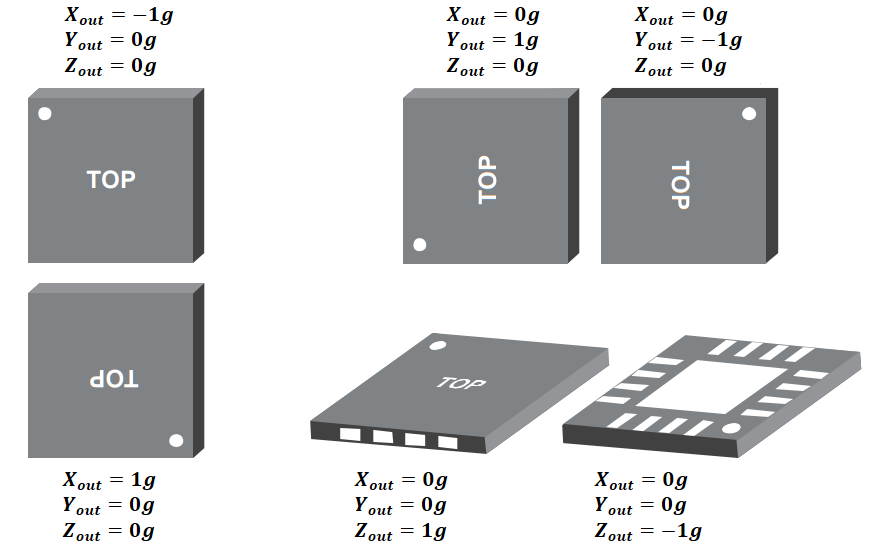
\includegraphics[width=0.85\textwidth]{figures/acc_paavirkning}
\caption{Påvirkning af accelerometeret i forskellige positioner. Til venstre måles accelerometeret lodret, til højre øverst vandret og til højre nederst i plan \citep{analogdevices2010}.}
\label{fig:acc}
\end{figure}

\noindent
Ved hældning af accelerometeret vil der ske en acceleration i forhold til tyngdekraften. Hvilken acceleration, der sker, er afhængigt af plan og hældningens retning. Dette fremgår af \autoref{fig:acc}. Herved vil der ske en ændring i outputspændingen ved en hældning på $0^{\circ}$. Hvis accelerometeret eksempelvis befinder sig i den øverste situation på \autoref{fig:acc}, påvirkes y-aksen med $-1~g$ \citep{clifford2005}. Denne sammenhæng og derved patientens hældning kan udtrykkes ved \autoref{equ:vinkler}, hvor $\phi$ er vinklen i forhold til udgangspunktet for den pågældende akse \citep{clifford2005}.

\begin{equation} \label{equ:vinkler}
	V_{out} = V_{offset} + sensitivitet \cdot \sin(\phi) \\
\end{equation}

\noindent
